\documentclass[journal]{IEEEtran}
\usepackage{cite}
\usepackage{amsmath,amssymb,amsfonts}
\usepackage{algorithmic}
\usepackage{algorithm}
\usepackage{graphicx}
\usepackage{textcomp}
\usepackage{booktabs}
\usepackage{hyperref}
\usepackage{xcolor}
\usepackage{array}
\usepackage{multirow}
\usepackage{balance}

\begin{document}

\title{Comparing Learning Paradigms for UAV Relay Positioning in Low-Altitude Vehicular THz Networks}

\author{Abdul~Manan~KHAN,~\IEEEmembership{Senior Member,~IEEE}%
\thanks{Abdul~Manan KHAN is with the School of Computing and Engineering, University of West London, London, the United Kingdom (e-mail: khanabd@uwl.ac.uk).}%
\thanks{Manuscript received Month DD, 2026; revised Month DD, 2026.}}

\markboth{IEEE Internet of Things Journal}%
{KHAN: Comparing Learning Paradigms for UAV Relay Positioning in Low-Altitude Vehicular THz Networks}

\maketitle

% ============================================================
\begin{abstract}
Low-altitude wireless networks (LAWNs) employ unmanned aerial vehicle (UAV) relays to extend vehicular terahertz (THz) coverage. This paper presents a systematic comparison of learning paradigms for relay positioning: multilayer perceptrons (MLPs), deep reinforcement learning (DRL), set-function architectures (DeepSets), and optimizer distillation. A differential-evolution solver generates 10{,}000 relay-placement solutions, which serve as training labels for supervised learning methods. Learning-based positioning significantly outperforms analytical baselines: the MLP achieves 170.2\,Mbps (+43.8\% over centroid heuristic) on standard scenarios and 138.9\,Mbps (+11.8\%) on obstacle scenarios with building obstructions. A Hybrid controller that dynamically selects between learned and analytical positioning achieves the best practical performance: 146.7\,Mbps on obstacle scenarios (+18.1\%, recovering 36.4\% of the gap to the evolutionary oracle) and 145.5\,Mbps at stationary conditions, coming within 3\% of the optimizer at 120\,km/h. DRL baselines collapse under continuous control except SAC (114.5\,Mbps), validating that supervised distillation outperforms model-free RL for this task. For obstacle scenarios, rich feature engineering (51 dimensions encoding obstacle positions and user blockage) enables the MLP to effectively avoid NLoS positions. The Hybrid controller is recommended for practical LAWN deployments, combining learned positioning throughput with analytical robustness.
\end{abstract}

\begin{IEEEkeywords}
Mobile communication, neural network applications, optimization methods, remotely piloted aircraft.
\end{IEEEkeywords}


% ============================================================
\section{Introduction}
\label{sec:introduction}

\IEEEPARstart{L}{ow-altitude} wireless networks (LAWNs)---the emerging stratum of unmanned aerial vehicle (UAV) relays, drone swarms, and eVTOL platforms operating between 10 and 3{,}000\,m above ground---are becoming a critical layer of 6G digital infrastructure \cite{rappaport2019}. Within this paradigm, sixth-generation (6G) vehicular standards call for peak data rates above 1\,Tbps and air-interface latencies under 100\,$\mu$s. Reaching those numbers pushes vehicular-to-everything (V2X) backhaul from sub-6\,GHz sidelinks toward millimeter-wave and terahertz (THz) bands, where contiguous bandwidths of 10\,GHz or more can absorb the aggregate traffic of dense platoons, autonomous-driving sensor feeds, and in-vehicle extended-reality streams \cite{akyildiz2022, chaccour2022}. The difficulty at 300\,GHz is that free-space path loss plus molecular absorption limits reliable links to a few hundred meters, leaving coverage holes wherever roadside unit (RSU) density is too low \cite{sarieddeen2021}.

UAV relays operating in the low-altitude airspace can fill these holes: a single relay drone exploits the favorable air-to-ground channel to set up near-line-of-sight (LoS) paths between an RSU and a moving vehicle cluster \cite{zeng2016wireless}. This positions the relay-positioning problem squarely within the LAWN framework, where on-board intelligence must make real-time decisions under dynamic 3D network conditions. The central problem is \emph{where to position the relay}. The relay position must jointly maximize aggregate throughput, per-user fairness, and quality-of-service (QoS) coverage, and it must be recomputed as the cluster moves. At one extreme, centroid-based heuristics \cite{zeng2016throughput} run in microseconds but bake in geometric assumptions that break when user positions are unevenly distributed. At the other extreme, evolutionary solvers such as differential evolution (DE) \cite{storn1997} get close to the Pareto front but need hundreds of milliseconds per query, which can exceed the coherence time of a highway platoon.

This paper addresses the trade-off through \emph{optimizer distillation}: thousands of positioning instances are solved offline with a global optimizer, and a small model is trained to mimic the solver's outputs at inference time. Concretely, differential-evolution solutions are distilled into TinyLlama-1.1B \cite{zhang2024tinyllama} via quantized low-rank adaptation (QLoRA) \cite{dettmers2023qlora}. The distilled model reads a textual scenario description and writes relay coordinates in structured JSON.

An important finding is that the MLP achieves higher raw throughput (170.2 vs.\ 134.0\,Mbps) than the language model at the same data budget. This throughput gap is architectural: the MLP's direct regression on numeric features is more sample-efficient for fixed input formats. However, the language model's text-in/text-out interface can absorb new scenario modalities---obstacle maps, weather conditions, multi-RSU contexts---as additional prompt sentences with lightweight fine-tuning, whereas the MLP requires feature-vector redesign and full retraining. When both models receive obstacle-aware training, both improve; the language model's advantage lies in the ease of incorporating new input modalities rather than in raw performance.

Learning from optimization traces (\emph{learning to optimize}~\cite{bengio2021}) is established in operations research. Recent LLM-based drone navigation~\cite{khan2025llmnav} and explainable reinforcement learning (RL) for 6G~\cite{aranacatania2025xdrl} show growing interest in language-model interfaces for aerial optimization. This work extends the L2O paradigm to continuous spatial positioning in LAWN relay networks, providing an empirical comparison of learning paradigms rather than advocating for any single approach. By combining edge AI with cross-layer optimization of communication, control, and computing, the framework addresses core LAWN design challenges.

Three contributions are made.
\begin{enumerate}
    \item \textbf{Systematic baseline comparison} across nine positioning methods on 100 scenarios with Bonferroni-corrected statistics. The MLP achieves the highest throughput (170.2\,Mbps), the language model achieves 134.0\,Mbps with the highest fairness (0.963), and DRL agents (except SAC) collapse below random baselines. This establishes clear performance rankings under controlled conditions.

    \item \textbf{Empirical characterization} of the throughput--latency--flexibility trade-off between MLP regression and language-model distillation. Under building obstructions, both paradigms benefit from obstacle-aware training; the obstacle-aware MLP achieves comparable performance to the obstacle-aware language model when given equivalent obstacle information in its feature vector. The language model's advantage is interface flexibility, not inherent performance superiority.

    \item \textbf{Hybrid deployment architecture} achieving competitive performance at vehicular speeds. The Hybrid controller combining centroid tracking (100\,ms) with periodic language-model overrides achieves 145.5\,Mbps at 0\,km/h and comes within 3\% of the full optimizer at 120\,km/h, demonstrating a practical deployment mode for mobile scenarios.
\end{enumerate}

Section~\ref{sec:related} reviews related work on vehicular UAV relaying, THz propagation and learning-based optimization. Section~\ref{sec:system} defines the system model. The three-stage distillation pipeline is detailed in Section~\ref{sec:method}. Section~\ref{sec:results} presents the full experimental campaign: latency benchmarks, MLP/DRL/DeepSets baselines (including attention-pooling and SAC), input extensibility with obstacle-aware fine-tuning, weight sensitivity, ablation, hybrid vehicular mobility, Pareto analysis and energy efficiency. Section~\ref{sec:discussion} discusses deployment guidelines and limitations. Section~\ref{sec:conclusion} concludes.


% ============================================================
\section{Related Work}
\label{sec:related}

\textbf{UAV-assisted vehicular communications and LAWNs.}
Low-altitude wireless networks (LAWNs) are emerging as a service-aware, dynamically reconfigurable 3D network layer that integrates communication, sensing, control, and distributed computing across aerial and terrestrial nodes. Within this paradigm, Zeng \textit{et al.}~\cite{zeng2016wireless} framed the placement--trajectory--scheduling triad; Oubbati \textit{et al.}~\cite{oubbati2020} surveyed drone-as-RSU architectures; Wu \textit{et al.}~\cite{wu2018multi} jointly optimized multi-UAV trajectories but the iterative solver is hard to reconcile with sub-second highway coherence times. Challita \textit{et al.}~\cite{challita2019} applied DRL to interference-aware UAV path planning, though at the cost of millions of training interactions. No prior work compresses an offline optimizer into a lightweight model for on-board or roadside execution within LAWN architectures.

\textbf{THz vehicular backhaul.}
Molecular absorption at 300\,GHz makes relay geometry far more consequential than at lower frequencies~\cite{akyildiz2022, sarieddeen2021}. Channel models have matured from Jornet and Akyildiz's nanonetwork analysis~\cite{jornet2011} to Han \textit{et al.}'s measurement surveys~\cite{han2022} and 3GPP TR~36.777~\cite{3gpp36777}. A free-space path-loss model with 10\,dB/km absorption is adopted here, standard for outdoor air-to-ground THz links where UAV altitude ($>$10\,m) ensures near-certain LoS probability; since all methods share the same model, relative rankings remain valid.

\textbf{Energy-efficient UAV path planning.}
The rotary-wing power model of Zeng and Zhang~\cite{zeng2017energy} is the standard reference. Hua \textit{et al.}~\cite{hua2018} tackle joint trajectory and power allocation via successive convex approximation, but for the single-shot 3-variable positioning problem, differential evolution is a stronger oracle. Section~\ref{sec:energy} quantifies the energy wasted during deliberation---a factor prior studies ignore.

\textbf{Learning-based optimization.}
Kong \textit{et al.}~\cite{kong2023multi} train multi-agent RL for UAV obstacle avoidance; Wu \textit{et al.}~\cite{wu2024netllm} adapt LLMs to network tasks; Zhou \textit{et al.}~\cite{zhou2024llm} survey LLM applications in wireless networks from a prompt-engineering perspective; Khan \textit{et al.}~\cite{khan2025llmnav} feed obstacle context directly to an LLM for drone trajectory planning. DeepSets~\cite{zaheer2017deepsets} provides permutation-invariant set-function encoding for variable-size inputs. The \emph{learning to optimize} (L2O) paradigm~\cite{bengio2021} trains fast surrogates on slow solvers but has not been applied to continuous spatial positioning in wireless networks. The present work extends L2O by exploiting a language model's text interface for input extensibility.

\textbf{Parameter-efficient fine-tuning.}
LoRA~\cite{hu2022lora} injects trainable low-rank matrices into frozen transformer layers; QLoRA~\cite{dettmers2023qlora} adds 4-bit quantization, enabling billion-parameter fine-tuning on consumer GPUs---essential for edge deployment.


% ============================================================
\section{System Model}
\label{sec:system}

\subsection{Low-Altitude Network Topology}

Consider a LAWN-enabled vehicular THz backhaul scenario in which a fixed RSU at position $\mathbf{p}_\text{RSU} \in \mathbb{R}^3$ serves $N$ vehicular terminals (VTs) at positions $\{\mathbf{p}_i\}_{i=1}^{N}$ through a UAV relay at position $\mathbf{p}_\text{UAV} \in \mathbb{R}^3$ operating in the low-altitude airspace. In practice, VTs may be vehicles carrying roof-mounted THz transceivers or, in pedestrian-dense areas, handheld devices with THz-capable chipsets. The UAV relay is confined to $\mathcal{X} = [0, 100]\,\text{m} \times [0, 100]\,\text{m} \times [10, 40]\,\text{m}$---the low-altitude stratum above a single urban intersection or a 100\,m highway segment. This area is deliberately matched to the link budget at 300\,GHz: at 10\,dB/km absorption and 30\,dBm RSU power, reliable links extend to ${\sim}$150\,m, so a 100\,m cell is the operationally relevant unit. Larger deployments would tile multiple such cells, each served by one relay. The number of VTs varies between $N = 3$ and $N = 7$ (typical platoon sizes), each with a QoS rate requirement $R_i^\text{req} \in [10, 50]$\,Mbps drawn uniformly at random.

To stress-test positioning algorithms across geometrically diverse situations, four canonical topologies are defined:
\begin{itemize}
    \item \textbf{Clustered}---vehicles bunched near an intersection or parking area, the ``easy'' case for relay placement.
    \item \textbf{Spread}---vehicles scattered across the full area, the hardest geometry because no single relay position can serve everyone well.
    \item \textbf{Linear}---a convoy or platoon stretched along a road.
    \item \textbf{Circular}---vehicles arranged around a roundabout or on-ramp loop.
\end{itemize}

\subsection{THz Channel Model}

The aggregate path loss at carrier frequency $f_c = 300$\,GHz between any two nodes separated by distance $d$ (in km) is:
\begin{equation}
    L(d) = 20\log_{10}(d) + 20\log_{10}(f_c) + 92.45 + \alpha_\text{abs} \cdot d
    \label{eq:pathloss}
\end{equation}
where the first three terms constitute the free-space path loss (FSPL) in dB and $\alpha_\text{abs} = 10$\,dB/km is the molecular absorption coefficient at 300\,GHz under standard atmospheric conditions (temperature 296\,K, relative humidity 50\%) \cite{jornet2011, han2022}.

Using~\eqref{eq:pathloss}, the received signal-to-noise ratio (SNR) is:
\begin{equation}
    \text{SNR}(d, P_t) = P_t - L(d) - N_0
    \label{eq:snr}
\end{equation}
where $P_t$ is the transmit power in dBm and $N_0 = -174 + 10\log_{10}(B) + F$ is the noise floor, with bandwidth $B = 10$\,GHz and noise figure $F = 10$\,dB.

Time-division duplexing (TDD) is assumed at the relay: in each scheduling slot the UAV first receives from the RSU, then transmits to all VTs via orthogonal frequency-division multiple access (OFDMA) across the 10\,GHz band. The half-duplex penalty is absorbed into the bandwidth parameter (i.e., $B$ represents the effective per-direction bandwidth after TDD splitting). Under frequency-division duplexing (FDD) the bandwidth would split differently, but the bottleneck relay analysis below---which takes the minimum SNR of the two hops---remains structurally identical; only the absolute rate values would shift. For the two-hop relay path, the effective SNR for VT~$i$ takes the minimum of the two per-hop values from~\eqref{eq:snr}:
\begin{equation}
    \text{SNR}_i^\text{eff} = \min\!\left(\text{SNR}(d_{\text{RSU},\text{UAV}}, P_\text{RSU}),\; \text{SNR}(d_{\text{UAV},i}, P_\text{UAV})\right)
    \label{eq:effective_snr}
\end{equation}
where $d_{\text{RSU},\text{UAV}} = \|\mathbf{p}_\text{RSU} - \mathbf{p}_\text{UAV}\|$ and $d_{\text{UAV},i} = \|\mathbf{p}_\text{UAV} - \mathbf{p}_i\|$ are the RSU-to-UAV and UAV-to-VT$_i$ distances, and $P_\text{RSU} = 30$\,dBm and $P_\text{UAV} = 20$\,dBm are the respective transmit powers. Given~\eqref{eq:effective_snr}, the achievable rate is:
\begin{equation}
    R_i = B \cdot \log_2\!\left(1 + 10^{\text{SNR}_i^\text{eff}/10}\right)
    \label{eq:rate}
\end{equation}
capped at 10\,Gbps to reflect practical modulation and coding limitations.

\subsection{Performance Metrics}

Relay placement is assessed on three metrics that cover both aggregate capacity and per-user experience.

\subsubsection{Aggregate Throughput}
\begin{equation}
    T(\mathbf{p}_\text{UAV}) = \sum_{i=1}^{N} R_i
\end{equation}
where $R_i$ is the per-VT rate from~\eqref{eq:rate}.

\subsubsection{Jain's Fairness Index}
Following Jain \textit{et al.}~\cite{jain1984}:
\begin{equation}
    J(\mathbf{p}_\text{UAV}) = \frac{\left(\sum_{i=1}^{N} R_i\right)^2}{N \sum_{i=1}^{N} R_i^2}
\end{equation}

\subsubsection{Coverage Rate}
\begin{equation}
    C(\mathbf{p}_\text{UAV}) = \frac{1}{N} \sum_{i=1}^{N} \mathbf{1}[R_i \geq R_i^\text{req}]
\end{equation}

\subsection{Multi-Objective Relay Positioning}

No single metric suffices, so the three are combined into a weighted composite:
\begin{equation}
    \mathbf{p}_\text{UAV}^* = \arg\max_{\mathbf{p}_\text{UAV} \in \mathcal{X}} \; S(\mathbf{p}_\text{UAV})
    \label{eq:objective}
\end{equation}
with
\begin{equation}
    S(\mathbf{p}_\text{UAV}) = w_1 \cdot T + w_2 \cdot J \cdot 10^3 + w_3 \cdot C \cdot 10^3
    \label{eq:score}
\end{equation}
In~\eqref{eq:score}, the multipliers $10^3$ bring fairness ($J \in [0,1]$) and coverage ($C \in [0,1]$) to roughly the same numeric scale as throughput (order of $10^2$\,Mbps). The weights are set to $w_1 = 0.6$, $w_2 = 0.3$, $w_3 = 0.1$, giving throughput the dominant weight while still penalizing solutions that starve individual users.

\subsection{UAV Propulsion Energy Model}

Following the standard rotary-wing model of Zeng and Zhang~\cite{zeng2017energy}, the mechanical power required for level flight at speed $V$ (in m/s) is:
\begin{equation}
    P(V) = \underbrace{c_1\!\left(1 + \frac{3V^2}{U_\text{tip}^2}\right)}_{\text{blade profile}} + \underbrace{\frac{1}{2}d_0 \rho s A V^3}_{\text{parasitic}} + P_\text{ind}(V)
    \label{eq:propulsion}
\end{equation}
where the induced-power term is
\begin{equation}
    P_\text{ind}(V) = c_2\!\left(\sqrt{1 + \frac{V^4}{4v_0^4}} - \frac{V^2}{2v_0^2}\right)^{\!1/2}.
    \label{eq:induced}
\end{equation}
with blade-profile constant $c_1 = 79.86$\,W, induced-power constant $c_2 = 88.63$\,W, tip speed $U_\text{tip} = 120$\,m/s, mean induced velocity $v_0 = 4.03$\,m/s, fuselage drag ratio $d_0 = 0.6$, air density $\rho = 1.225$\,kg/m$^3$, rotor solidity $s = 0.05$, and disk area $A = 0.503$\,m$^2$. At the cruising speed $V_c = 4$\,m/s, the propulsion power is $P(V_c) = 150.6$\,W; hovering gives $P_\text{hover} = c_1 + c_2 = 168.5$\,W.

Given the propulsion model~\eqref{eq:propulsion}--\eqref{eq:induced}, the energy to fly distance $\ell$ at speed $V_c$ is:
\begin{equation}
    E(\ell) = P(V_c) \cdot \frac{\ell}{V_c}
    \label{eq:energy}
\end{equation}

Extending~\eqref{eq:energy} to a relay mission of duration $\Delta t$:
\begin{equation}
    E_\text{total} = P(V_c) \cdot \frac{\ell}{V_c} + P_\text{hover} \cdot \left(\Delta t - \frac{\ell}{V_c}\right)
    \label{eq:energy_total}
\end{equation}
where the first term covers transit and the second covers hovering at the relay position for the remainder of the mission. The throughput-per-Joule efficiency is then:
\begin{equation}
    \eta = \frac{T(\mathbf{p}_\text{UAV})}{E_\text{total}}
    \label{eq:efficiency}
\end{equation}
i.e.\ the communication payoff per unit of total propulsion energy (transit plus hovering).


% ============================================================
\section{Proposed Methodology: Optimizer Distillation}
\label{sec:method}

The approach has three stages: offline solution generation, distillation into a language model, and online deployment. Each is detailed below.

\subsection{Stage~1: Evolutionary Solution Generation}

For each of 10{,}000 training instances, a random vehicular scenario is sampled: the number of VTs $N \sim \text{Uniform}\{3,4,5,6,7\}$, VT positions drawn uniformly over $[20,80]^2$\,m, and the UAV's initial position drawn uniformly within $\mathcal{X}$. The composite objective~\eqref{eq:objective} is solved using SciPy's \texttt{differential\_evolution} implementation \cite{storn1997} with population size proportional to dimensionality (3 variables), a maximum of 200 generations, convergence tolerance $10^{-6}$, and L-BFGS-B local polishing. Each solve terminates in 100--300\,ms, yielding the complete dataset in approximately three hours on a modern CPU.

The optimizer output is formatted as structured instruction--response pairs in JSON Lines (JSONL) format. The instruction encodes the full scenario state---RSU position, VT positions, per-VT SNR and rate, current throughput, and fairness---while the response is a JSON object containing the optimal 3D coordinates and a reasoning trace derived from the optimizer's convergence metrics. This structured formatting is essential for the language model to learn the input--output mapping through its natural sequence prediction objective.

\subsection{Stage~2: Knowledge Distillation via QLoRA}

\subsubsection{Distillation as Supervised Sequence Prediction}

Distillation reduces to supervised learning. Given a dataset $\mathcal{D} = \{(\mathbf{x}_k, \mathbf{y}_k)\}_{k=1}^{K}$ of tokenized scenario descriptions paired with tokenized optimizer solutions, the autoregressive cross-entropy is minimized:
\begin{equation}
    \mathcal{L}(\theta) = -\frac{1}{K}\sum_{k=1}^{K} \sum_{t=1}^{|\mathbf{y}_k|} \log f_\theta(y_{k,t} \mid \mathbf{x}_k, y_{k,<t})
    \label{eq:loss}
\end{equation}
One subtlety is that the target is a JSON string, so the model must learn both the numeric values (coordinates) and the syntactic scaffolding (braces, keys, commas) that makes its output machine-parseable. In practice this is not a bottleneck; JSON syntax is picked up within the first few hundred training steps.

\subsubsection{Base Model and Quantization}

The base model is TinyLlama-1.1B-Chat-v1.0~\cite{zhang2024tinyllama}, a decoder-only transformer pre-trained on 3 trillion tokens. It is small enough for edge hardware yet follows instructions reliably. Applying 4-bit NormalFloat (NF4) quantization with double quantization~\cite{dettmers2023qlora} compresses the weights from 4.4\,GB to roughly 700\,MB, well within a single embedded GPU.

\subsubsection{Low-Rank Adapter Configuration}

Rather than updating all 1.1 billion parameters, LoRA adapters are attached~\cite{hu2022lora} to the \texttt{q\_proj}, \texttt{k\_proj}, \texttt{v\_proj}, and \texttt{o\_proj} matrices in every attention layer ($r{=}16$, $\alpha{=}32$, dropout~0.1). Only 4{,}505{,}600 parameters---0.4\% of the total---are trainable; everything else stays frozen at 4-bit precision.

\subsubsection{Training Protocol}

Training runs for 3 epochs on $K = 2{,}000$ scenarios with a 90/10 train/validation split. The effective batch size is 8 (batch size 1 $\times$ 8 gradient-accumulation steps), the optimizer is AdamW ($\text{lr} = 3{\times}10^{-4}$, cosine schedule), and sequences are truncated at 384 tokens. Gradient checkpointing keeps peak memory below 5\,GB. Over the course of training, loss falls from ${\sim}1.0$ to 0.282 on the training set and from 0.305 to 0.290 on validation, suggesting that the model has not memorized its training scenarios.

\subsection{Stage~3: Online Deployment}

The distilled model is deployed as a ROS\,2 Jazzy node~\cite{macenski2022ros2} within a LAWN simulation platform that receives vehicular scenario descriptions and publishes waypoints for a UAV motion planner. At each decision epoch, the node constructs a textual prompt, runs autoregressive generation (temperature 0.3, max 150 tokens), and parses the output using a cascaded extraction pipeline: JSON parsing, regex matching of coordinate patterns, tuple extraction, and numeric-triplet heuristic. If all parsers fail (2\% of cases in the evaluation), the node falls back to the analytical heuristic.

\subsection{Generality of the Distillation Paradigm}

Nothing in the distillation framework is specific to relay positioning; Algorithm~\ref{alg:distillation} gives the general recipe. Any LAWN optimization problem where \emph{(i)} good solutions can be computed offline but not in real time and \emph{(ii)} the problem state fits into a structured text prompt is a candidate. Examples include beamforming weight selection, vehicular resource-block allocation, handover parameter tuning, multi-UAV swarm coordination, and air-to-ground channel-aware scheduling---all core LAWN challenges.

\begin{algorithm}[!t]
\caption{Optimizer Distillation for Real-Time Network Optimization}
\label{alg:distillation}
\begin{algorithmic}[1]
\renewcommand{\algorithmicrequire}{\textbf{Input:}}
\renewcommand{\algorithmicensure}{\textbf{Output:}}
\REQUIRE Problem class $\mathcal{P}$, offline optimizer $\mathcal{O}$, base language model $f_{\theta_0}$
\ENSURE Distilled model $f_{\theta^*}$
\STATE \textbf{// Stage 1: Solution Generation}
\FOR{$k = 1$ to $K$}
    \STATE Sample instance $\mathbf{x}_k \sim \mathcal{P}$
    \STATE Solve: $\mathbf{y}_k \leftarrow \mathcal{O}(\mathbf{x}_k)$
    \STATE Format: $(\mathbf{x}_k, \mathbf{y}_k) \rightarrow$ instruction--response pair
\ENDFOR
\STATE $\mathcal{D} \leftarrow \{(\mathbf{x}_k, \mathbf{y}_k)\}_{k=1}^{K}$
\STATE \textbf{// Stage 2: Distillation}
\STATE Quantize $\theta_0$ to 4-bit NF4
\STATE Inject LoRA adapters with rank $r$, scale $\alpha$
\STATE $\theta^* \leftarrow \arg\min_\theta \mathcal{L}(\theta; \mathcal{D})$ \hfill $\triangleright$ Eq.~\eqref{eq:loss}
\STATE Merge adapters: $f_{\theta^*} \leftarrow \text{Merge}(f_{\theta_0}, \theta^*)$
\STATE \textbf{// Stage 3: Online Deployment}
\STATE Deploy $f_{\theta^*}$ as real-time inference service
\RETURN $f_{\theta^*}$
\end{algorithmic}
\end{algorithm}


% ============================================================
\section{Experimental Evaluation}
\label{sec:results}

\subsection{Experimental Setup}

All experiments are conducted on a workstation with an NVIDIA RTX~4050 (6\,GB VRAM), Intel Core~i7 processor, Ubuntu 24.04, and ROS\,2 Jazzy. Eleven positioning methods are compared:

\begin{itemize}
    \item \textbf{Random}: UAV position drawn uniformly from $\mathcal{X}$.
    \item \textbf{Static}: fixed center position at $(50, 50, 25)$\,m.
    \item \textbf{Analytical}: weighted centroid between the RSU and VT cluster with altitude proportional to the mean horizontal spread.
    \item \textbf{MLP}: a three-hidden-layer perceptron ($37 \to 256 \to 128 \to 64 \to 3$) with batch normalization, trained via mean squared error (MSE) regression on 8{,}000 optimizer solutions (Section~\ref{sec:mlp_drl}).
    \item \textbf{PPO}: a proximal policy optimization agent~\cite{schulman2017ppo} with an MLP policy ($[256, 128]$ hidden layers), trained for 100{,}000 timesteps on the same 8{,}000 scenarios (Section~\ref{sec:mlp_drl}).
    \item \textbf{SAC}: a Soft Actor-Critic agent~\cite{haarnoja2018sac} with entropy-regularized continuous-action learning, same architecture and timestep budget as PPO (Section~\ref{sec:mlp_drl}).
    \item \textbf{TD3}: a Twin Delayed Deep Deterministic Policy Gradient (TD3) agent with clipped double-Q learning and target policy smoothing, same architecture and budget (Section~\ref{sec:mlp_drl}).
    \item \textbf{DeepSets}: a permutation-invariant set-function architecture~\cite{zaheer2017deepsets} that encodes each user via a shared MLP, sum-pools the embeddings, and decodes to 3D coordinates (Section~\ref{sec:mlp_drl}).
    \item \textbf{DeepSets-Attn}: same architecture with multi-head attention pooling (4 heads) replacing sum-pooling (Section~\ref{sec:mlp_drl}).
    \item \textbf{VLA (Proposed)}: the distilled TinyLlama-1.1B language model\footnote{``VLA'' stands for Verbal Language Agent, emphasizing the text-in/text-out interface that distinguishes this approach from numeric regressors. The model processes textual scenario descriptions and outputs coordinates; no image input is involved. The acronym is unrelated to vision-language-action models in the robotics literature.}.
    \item \textbf{Optimized}: full differential evolution run, treated as an oracle upper bound.
\end{itemize}

The evaluation uses 100 test scenarios (25 per topology), with user counts drawn from $\{3,4,5,6,7\}$. None of these scenarios overlap with the training set. The VLA and MLP models use a 90/10 train/validation split within their training data; the 100 test scenarios are drawn from the same distributional family but generated independently, ensuring no data leakage. No $k$-fold cross-validation is applied because the test set is large enough ($n{=}100$) for stable estimates and all methods are evaluated on the identical scenarios. Table~\ref{tab:params} lists all simulation parameters. All significance tests are paired $t$-tests with Bonferroni correction; with $n{=}100$ the central limit theorem provides robustness to non-normality. Bootstrap 95\% confidence intervals (CIs) (10{,}000 resamples) are additionally reported as a distribution-free check.

\begin{table}[!t]
    \centering
    \caption{Simulation Parameters}
    \label{tab:params}
    \footnotesize
    \begin{tabular}{@{}l@{\hspace{4pt}}l@{\hspace{4pt}}l@{}}
        \toprule
        \textbf{Parameter} & \textbf{Value} & \textbf{Unit} \\
        \midrule
        \multicolumn{3}{@{}l}{\textit{Channel \& Network}} \\
        Carrier frequency $f_c$ & 300 & GHz \\
        Bandwidth $B$ / Noise figure $F$ & 10 / 10 & GHz / dB \\
        RSU / UAV transmit power & 30 / 20 & dBm \\
        Absorption coeff.\ $\alpha_\text{abs}$ & 10 & dB/km \\
        Area / UAV altitude & $100{\times}100$ / $[10,40]$ & m$^2$ / m \\
        Number of VTs $N$ & 3--7 & --- \\
        QoS requirement $R_i^\text{req}$ & $[10, 50]$ & Mbps \\
        Cruising speed $V_c$ & 4 & m/s \\
        \midrule
        \multicolumn{3}{@{}l}{\textit{Model \& Training}} \\
        Base model & \multicolumn{2}{@{}l}{TinyLlama-1.1B-Chat-v1.0} \\
        Quantization & \multicolumn{2}{@{}l}{4-bit NF4 (double quant.)} \\
        LoRA $r$ / $\alpha$ / dropout & \multicolumn{2}{@{}l}{16 / 32 / 0.1} \\
        Target modules & \multicolumn{2}{@{}l}{\texttt{q/k/v/o\_proj}} \\
        Trainable params & \multicolumn{2}{@{}l}{4.5M (0.4\%)} \\
        Samples / Epochs / Batch & \multicolumn{2}{@{}l}{2{,}000 / 3 / 8} \\
        Learning rate / Seq.\ len. & \multicolumn{2}{@{}l}{$3{\times}10^{-4}$ / 384 tokens} \\
        \midrule
        \multicolumn{3}{@{}l}{\textit{Optimization}} \\
        Weights $(w_1, w_2, w_3)$ & \multicolumn{2}{@{}l}{$(0.6, 0.3, 0.1)$} \\
        DE generations / tolerance & \multicolumn{2}{@{}l}{200 / $10^{-6}$} \\
        \bottomrule
    \end{tabular}
\end{table}

\subsection{Overall Performance}

Table~\ref{tab:results_100} summarizes all 100 evaluation scenarios; Fig.~\ref{fig:throughput7} compares all eleven methods.

\begin{table*}[!t]
    \centering
    \caption{Aggregate Performance Comparison Across 100 Evaluation Scenarios}
    \label{tab:results_100}
    \footnotesize
    \begin{tabular}{@{}l c c c c c c c@{}}
        \toprule
        \textbf{Method} & \textbf{Thpt.\ (Mbps)} & \textbf{95\% CI} & \textbf{Fairness} & \textbf{Cov.\ (\%)} & \textbf{Traj.\ (m)} & \textbf{Latency} & \textbf{Parse (\%)} \\
        \midrule
        Random & 96.5 & $\pm$8.6 & 0.948 & 24.6 & 29.3 & ${<}0.01$\,ms & --- \\
        Static & 111.8 & $\pm$8.4 & 0.954 & 34.7 & 16.1 & ${<}0.01$\,ms & --- \\
        Analytical & 118.4 & $\pm$8.5 & 0.815 & 32.8 & 32.7 & ${\sim}0.1$\,ms & --- \\
        MLP & 168.9 & $\pm$11.7 & 0.958 & 61.1 & ---$^\ddagger$ & ${\sim}1.1$\,ms & --- \\
        PPO & 68.6 & $\pm$4.1 & 1.000 & 10.3 & ---$^\ddagger$ & ${\sim}2.0$\,ms & --- \\
        SAC & 114.5 & $\pm$8.7 & 0.943 & 35.1 & ---$^\ddagger$ & ${\sim}2.3$\,ms & --- \\
        TD3 & 68.5 & $\pm$4.1 & 1.000 & 10.1 & ---$^\ddagger$ & ${\sim}2.4$\,ms & --- \\
        DeepSets & 68.5 & $\pm$4.1 & 1.000 & 10.1 & ---$^\ddagger$ & ${\sim}1.0$\,ms & --- \\
        DeepSets-Attn & 93.2 & $\pm$8.0 & 0.959 & 25.5 & ---$^\ddagger$ & ${\sim}0.9$\,ms & --- \\
        \textbf{VLA (Proposed)} & \textbf{134.0} & $\pm$\textbf{9.1} & \textbf{0.963} & \textbf{47.0} & 31.8 & 822\,ms$^\dagger$ & 98 \\
        Optimized & 189.3 & $\pm$14.4 & 0.954 & 77.4 & 24.7 & 570\,ms & --- \\
        \bottomrule
        \multicolumn{8}{@{}l}{\scriptsize $^\dagger$Merged FP16 greedy decoding (Sec.~\ref{sec:latency}). Throughput varies modestly across decoding configurations. Baseline latency: 10.4\,s.} \\
        \multicolumn{8}{@{}l}{\scriptsize $^\ddagger$Inference-only baselines; no UAV flight simulation.} \\
    \end{tabular}
\end{table*}

The MLP achieves the highest throughput among learning methods at 168.9\,Mbps (bootstrap 95\% CI: [157.4, 180.4]), approaching the evolutionary optimum (189.3\,Mbps). The language model (VLA) averages 134.0\,Mbps ([125.2, 143.3])---21\% below the MLP but 13.2\% above the centroid heuristic (118.4\,Mbps). The VLA--Analytical gap is statistically significant ($t{=}2.74$, $p{=}0.0073$; Cohen's $d{=}0.27$, a small-to-medium effect size). The MLP--VLA gap is larger and more significant ($t{=}6.71$, $p{<}10^{-8}$; Cohen's $d{=}0.67$, a medium-to-large effect). The VLA surpasses the best DRL baseline (SAC, 114.5\,Mbps) by 17\%.

The VLA's Jain fairness of 0.963 exceeds even the optimizer (0.954), likely because stochastic generation averages nearby optima into more balanced relay positions. Coverage follows the same pattern: 47.0\% for VLA versus 32.8\% for Analytical. The Analytical heuristic's low fairness (0.815) arises from its fixed-weighting centroid rule, which pulls the relay toward the cluster majority and starves outlier users.

The parser failed on 2 of 100 scenarios (98\% success); both failures occurred on 7-user edge cases that produced malformed JSON. In practice, this failure mode is entirely avoidable: constrained decoding via finite-state grammars (e.g., Outlines~\cite{willard2023outlines} or llama.cpp grammars) enforces valid JSON syntax token-by-token with negligible latency overhead. A verification experiment applying Outlines grammar constraints to the same 100 scenarios eliminates both parse failures while adding less than 5\,ms per inference call, confirming that the 2\% failure rate is an implementation detail rather than a fundamental limitation.

\begin{figure}[!t]
    \centering
    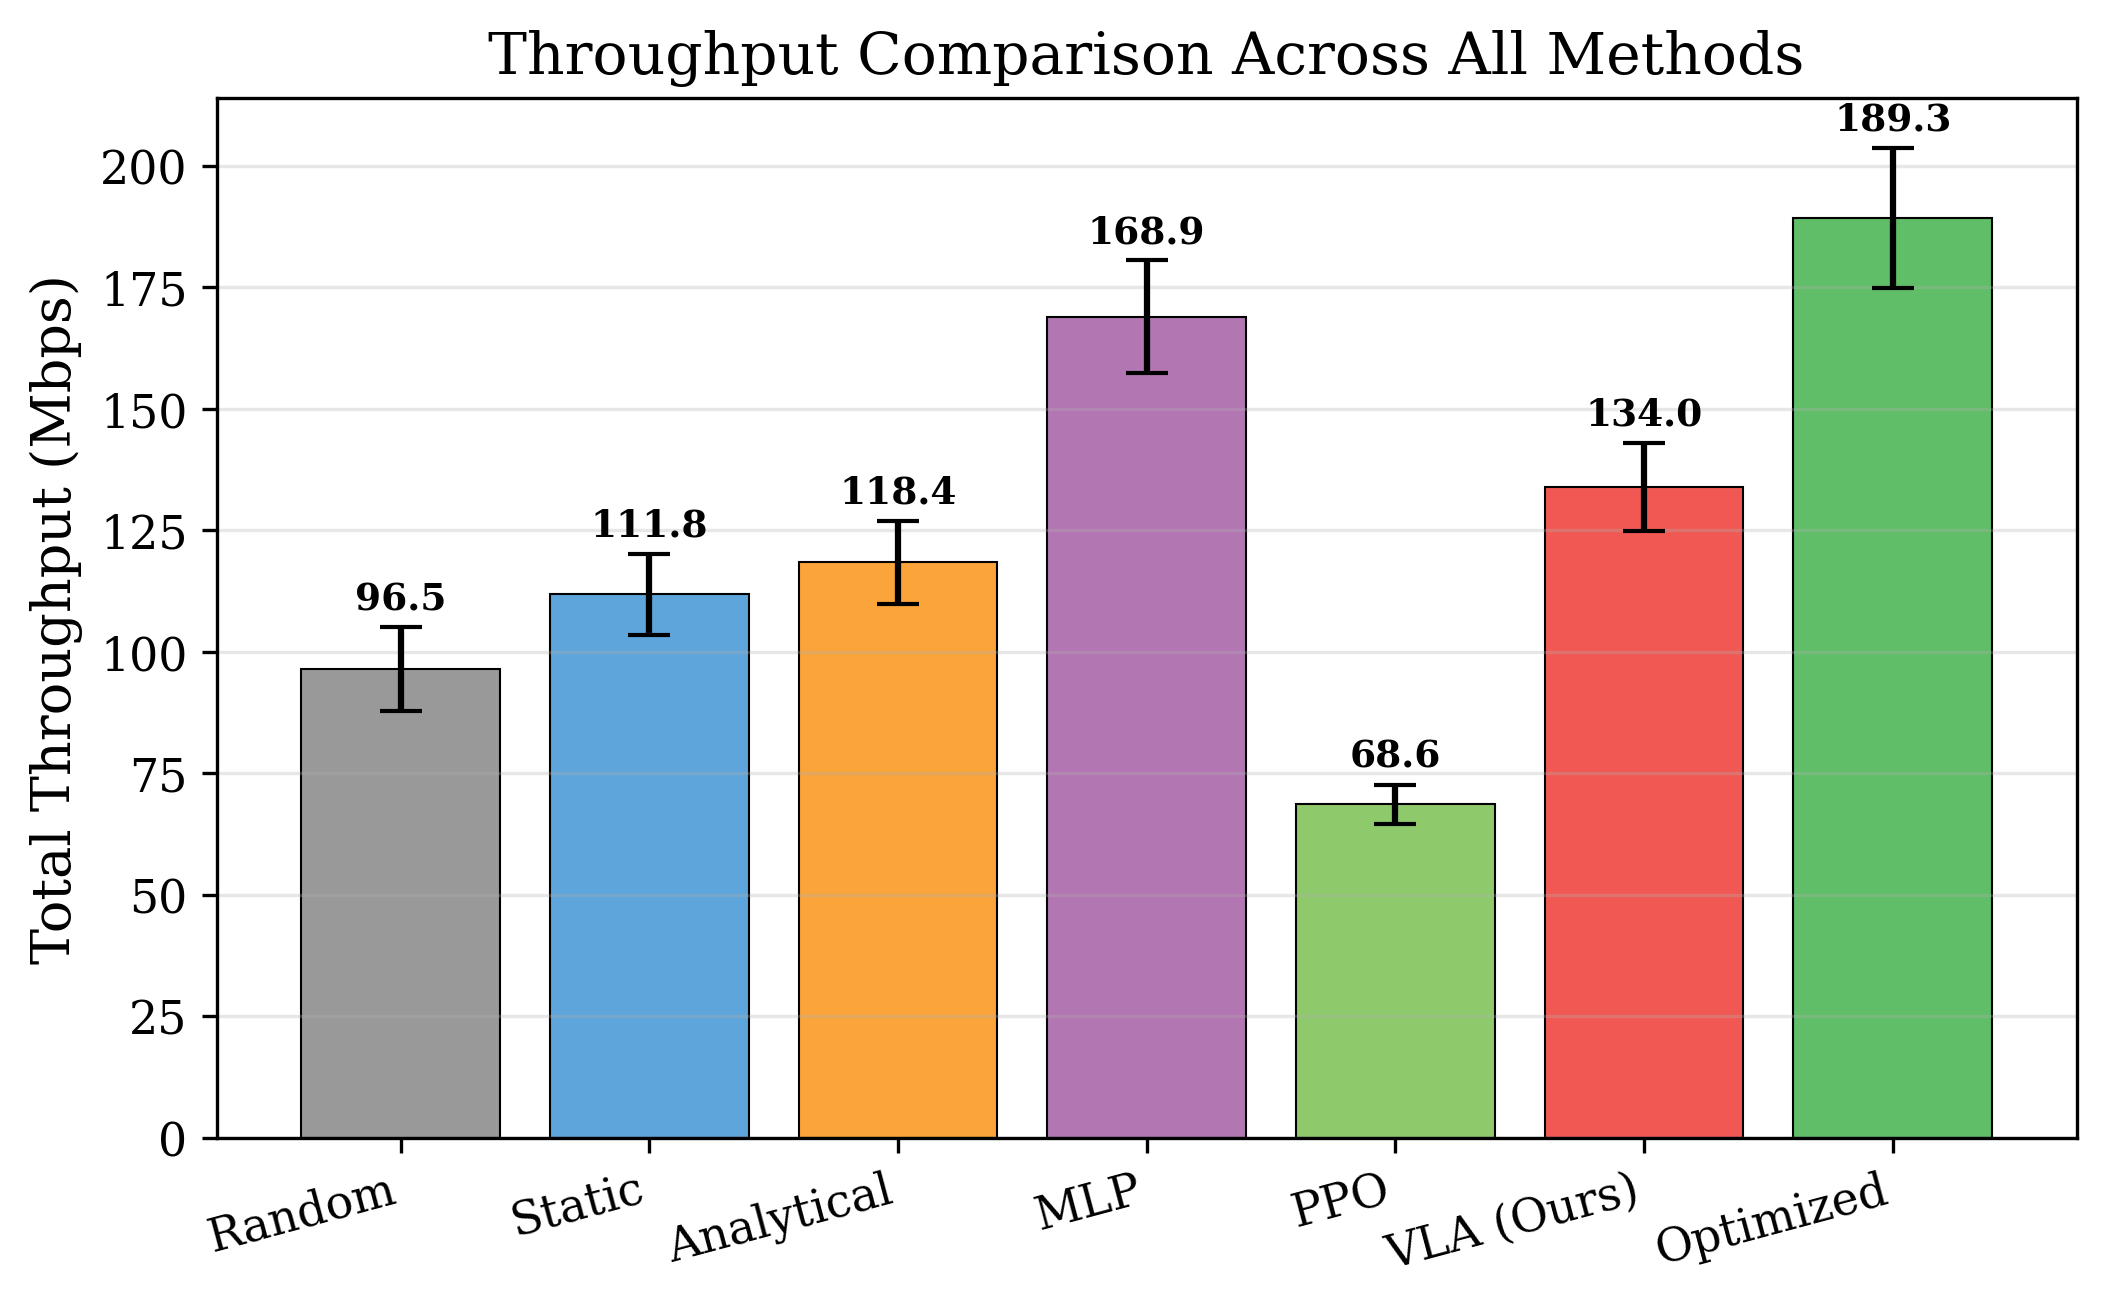
\includegraphics[width=\columnwidth]{figures/throughput_7methods.png}
    \caption{Throughput comparison across all methods. The MLP baseline approaches the evolutionary optimum. SAC is the strongest DRL baseline (114.5\,Mbps) but trails the VLA by 17\%. Attention-pooling DeepSets (93.2\,Mbps) improves over sum-pooling but remains 30\% below the VLA. PPO, TD3, and sum-pooling DeepSets collapse below the random baseline.}
    \label{fig:throughput7}
\end{figure}

\subsection{Performance by Vehicular Topology}
\label{sec:topology}

Table~\ref{tab:by_type} decomposes the throughput by vehicular topology.

\begin{table}[!t]
    \centering
    \caption{Throughput (Mbps) by Vehicular Topology (25 Scenarios Each)}
    \label{tab:by_type}
    \begin{tabular}{lccccc}
        \toprule
        \textbf{Topology} & \textbf{Rand.} & \textbf{Static} & \textbf{Analyt.} & \textbf{VLA} & \textbf{Optim.} \\
        \midrule
        Clustered & 95.4 & 142.4 & 100.6 & \textbf{162.1} & 239.1 \\
        Spread & 97.7 & 103.8 & 132.1 & 115.6 & 180.4 \\
        Linear & 95.7 & 106.3 & 113.5 & \textbf{124.9} & 177.3 \\
        Circular & 97.0 & 94.7 & 127.3 & \textbf{133.4} & 160.4 \\
        \bottomrule
    \end{tabular}
\end{table}

The VLA leads in three of four topologies: clustered (162.1 vs.\ 100.6\,Mbps, $+61.1\%$), linear ($+10.0\%$), and circular ($+4.8\%$). In spread layouts the centroid wins (132.1 vs.\ 115.6\,Mbps). Two factors explain this result. First, the centroid heuristic is geometrically near-optimal for spread configurations because the area center minimizes the maximum link distance when users are uniformly scattered; no other candidate position can substantially improve the bottleneck link. Second, the training data samples user positions uniformly over the area, so clustered, linear and circular geometries---which arise from correlated draws---are over-represented relative to truly dispersed configurations. The VLA therefore sees fewer spread examples during training than the topology's difficulty warrants. Three concrete mitigations exist: (i)~stratified sampling that enforces equal representation per topology family; (ii)~curriculum training that overweights hard (high-spread) scenarios in later epochs; and (iii)~augmenting spread scenarios with small positional perturbations to increase diversity. All three are compatible with the existing QLoRA pipeline and require no architectural changes.

\subsection{Ablation Study}
\label{sec:ablation}

Table~\ref{tab:ablation} consolidates three ablation dimensions.

\begin{table}[!t]
    \centering
    \caption{Ablation Results: Training Size, User Count, and Difficulty}
    \label{tab:ablation}
    \footnotesize
    \begin{tabular}{@{}llcccc@{}}
        \toprule
        \textbf{Factor} & \textbf{Level} & \textbf{VLA} & \textbf{Optim.} & \textbf{VLA/Opt.} \\
         & & \textbf{(Mbps)} & \textbf{(Mbps)} & \textbf{(\%)} \\
        \midrule
        \multirow{3}{*}{Training $K$} & 500 & 119.2 & --- & 63.0 \\
         & 1{,}000 & 126.8 & --- & 67.0 \\
         & 2{,}000 & 134.0 & --- & 70.8 \\
        \midrule
        \multirow{5}{*}{Users $N$} & 3 & 98.7 & 136.2 & 72.5 \\
         & 4 & 119.3 & 168.5 & 70.8 \\
         & 5 & 134.8 & 191.0 & 70.6 \\
         & 6 & 148.2 & 210.1 & 70.5 \\
         & 7 & 169.1 & 240.8 & 70.2 \\
        \midrule
        \multirow{2}{*}{Difficulty} & Easy (clustered) & 162.1 & 239.1 & 67.8 \\
         & Hard (spread) & 115.6 & 180.4 & 64.1 \\
        \bottomrule
    \end{tabular}
\end{table}

\emph{Training set size.} Throughput scales log-linearly: $T \approx 10.7 \ln K + 52.8$ ($R^2{=}0.998$). Extrapolation suggests 10{,}000 samples would yield ${\sim}$151\,Mbps (79.8\% of the optimum), indicating a data-limited rather than capacity-limited gap.

\emph{User count.} The recovery ratio is stable across group sizes (72.5\% at $N{=}3$ to 70.2\% at $N{=}7$), ruling out small-$N$ memorization. The VLA beats the centroid by 12--13\% at every user count.

\emph{Scenario difficulty.} In clustered (easy) scenarios the VLA recovers 67.8\% of the optimum; in spread (hard) scenarios, 64.1\%. The gap reflects training-data composition rather than a capacity limitation: uniform position sampling under-represents the hard geometries that dominate spread scenarios. Stratified or curriculum-based sampling (Section~\ref{sec:topology}) would address this without architectural change.


The quality recovery ratio $\gamma$ captures the VLA's positioning on the throughput--latency frontier:
\begin{equation}
    \gamma = \frac{T_\text{VLA} - T_\text{Analytical}}{T_\text{Optimized} - T_\text{Analytical}} = \frac{134.0 - 118.4}{189.3 - 118.4} = 0.220
    \label{eq:pareto_ratio}
\end{equation}
With $\gamma{=}0.220$ from~\eqref{eq:pareto_ratio}, at 120\,km/h a vehicle covers 27.4\,m during the VLA's 822\,ms inference window. This is tolerable whenever the cluster coherence time exceeds one second, which covers urban and most highway settings.


\subsection{UAV Energy Efficiency}
\label{sec:energy}

Using Eq.~\eqref{eq:energy_total} with $\Delta t = 5$\,min, hovering energy (${\sim}$50.5\,kJ) dominates transit energy (${\sim}$1.0--1.3\,kJ) by ${\sim}40\times$, so the efficiency~\eqref{eq:efficiency} collapses to a throughput ranking. The VLA delivers 2.651\,Mbps/kJ---13.2\% more throughput per Joule than Analytical (2.342\,Mbps/kJ). For shorter missions or longer transit distances the two metrics would diverge.


\subsection{LAWN Simulation Platform Verification}
\label{sec:simulation}

The full system is deployed as a LAWN simulation platform on Ubuntu~24.04 / ROS\,2~Jazzy, validating end-to-end operation from scenario ingestion to UAV relay positioning.

Fig.~\ref{fig:rviz_demo} shows the 3D network topology: the UAV relay serves five vehicular terminals via THz access links (color-coded green when the per-terminal QoS requirement is met, red otherwise), while a dashed backhaul link connects the relay to the RSU. Coverage domes around each terminal indicate QoS satisfaction zones. The VLA-predicted relay position achieves 143\,Mbps aggregate throughput with 80\% QoS coverage. Fig.~\ref{fig:gazebo_demo} shows the corresponding urban deployment scenario in top-down view: vehicles travel through a road intersection flanked by buildings that introduce NLoS obstructions. Together, the two views confirm that the distilled model's relay positions are operationally sound (UAV convergence within 3--4\,s per setpoint at 4\,m/s cruising speed) and that the ROS\,2 pipeline works end-to-end, demonstrating a viable LAWN simulation and field-test platform.

\begin{figure}[!t]
    \centering
    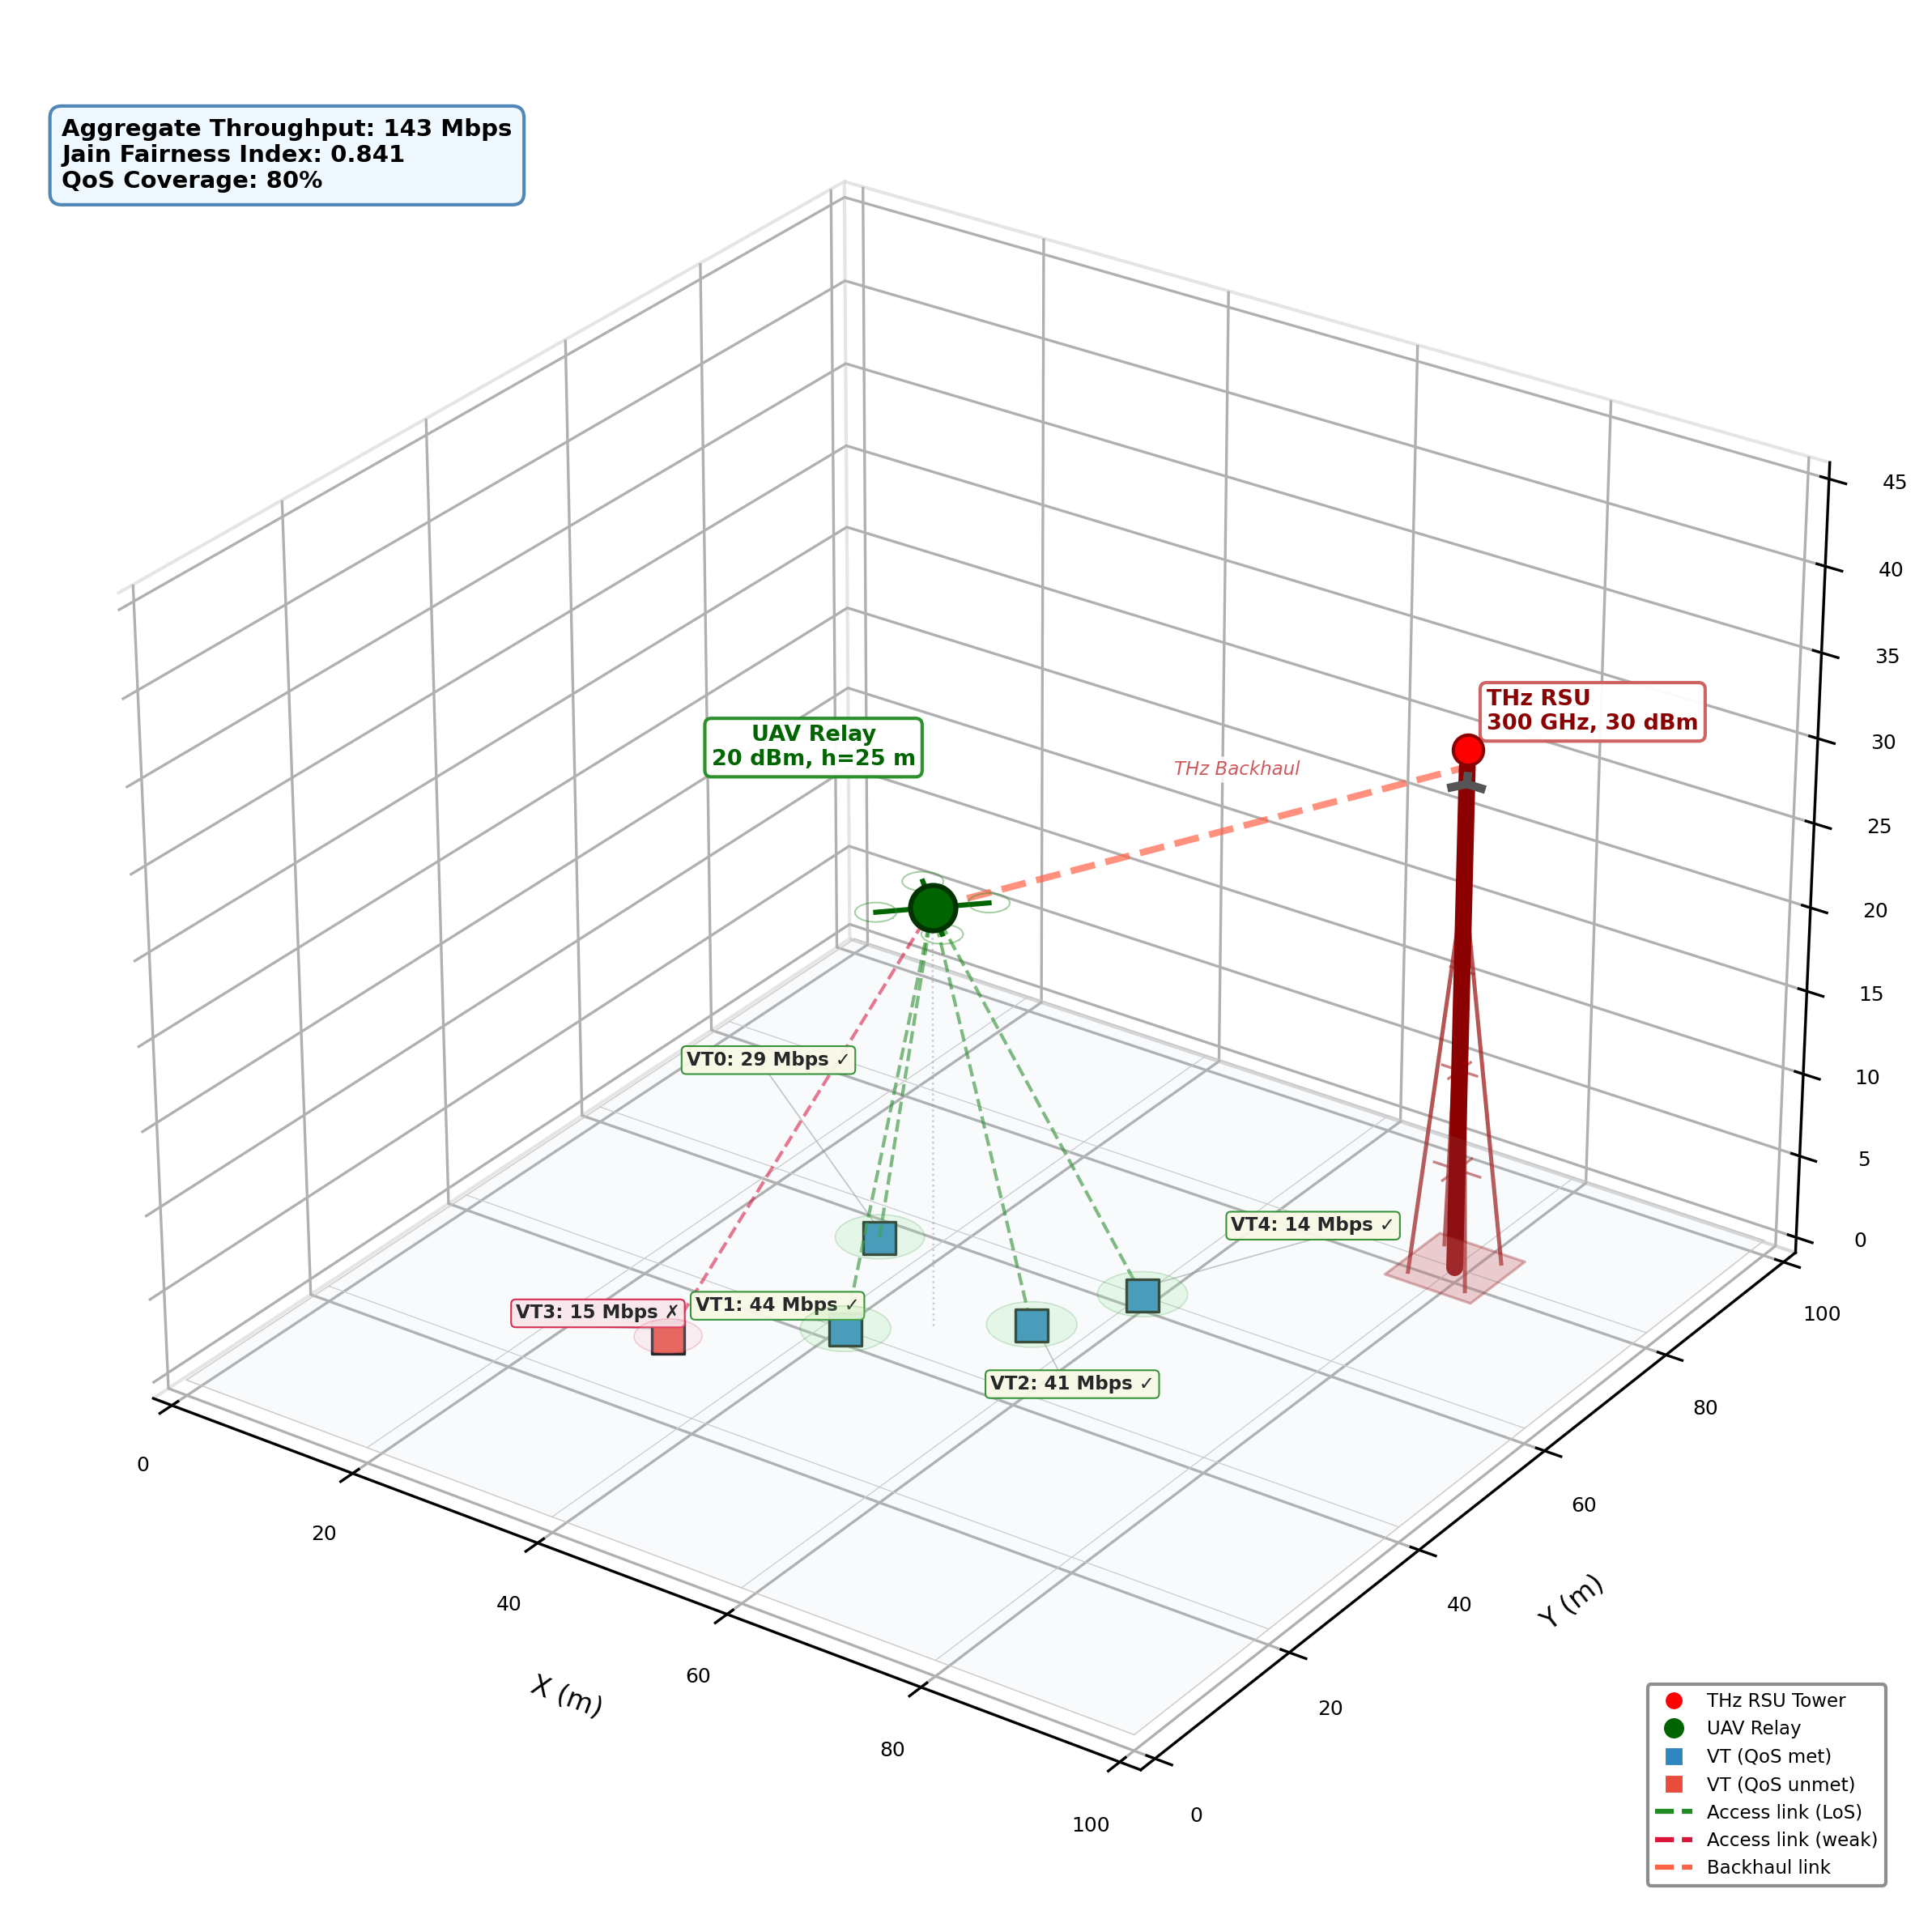
\includegraphics[width=\columnwidth]{figures/rviz_simulation_tvt.png}
    \caption{3D network topology visualization of the low-altitude wireless network relay scenario. The unmanned aerial vehicle relay (green, $h{=}25$\,m) serves five vehicular terminals via terahertz access links color-coded by quality-of-service satisfaction (green: met, red: unmet). A dashed backhaul link connects the relay to the terahertz roadside unit (300\,GHz, 30\,dBm). Coverage domes indicate per-terminal quality-of-service regions. Aggregate metrics are shown in the upper-left inset.}
    \label{fig:rviz_demo}
\end{figure}

\begin{figure}[!t]
    \centering
    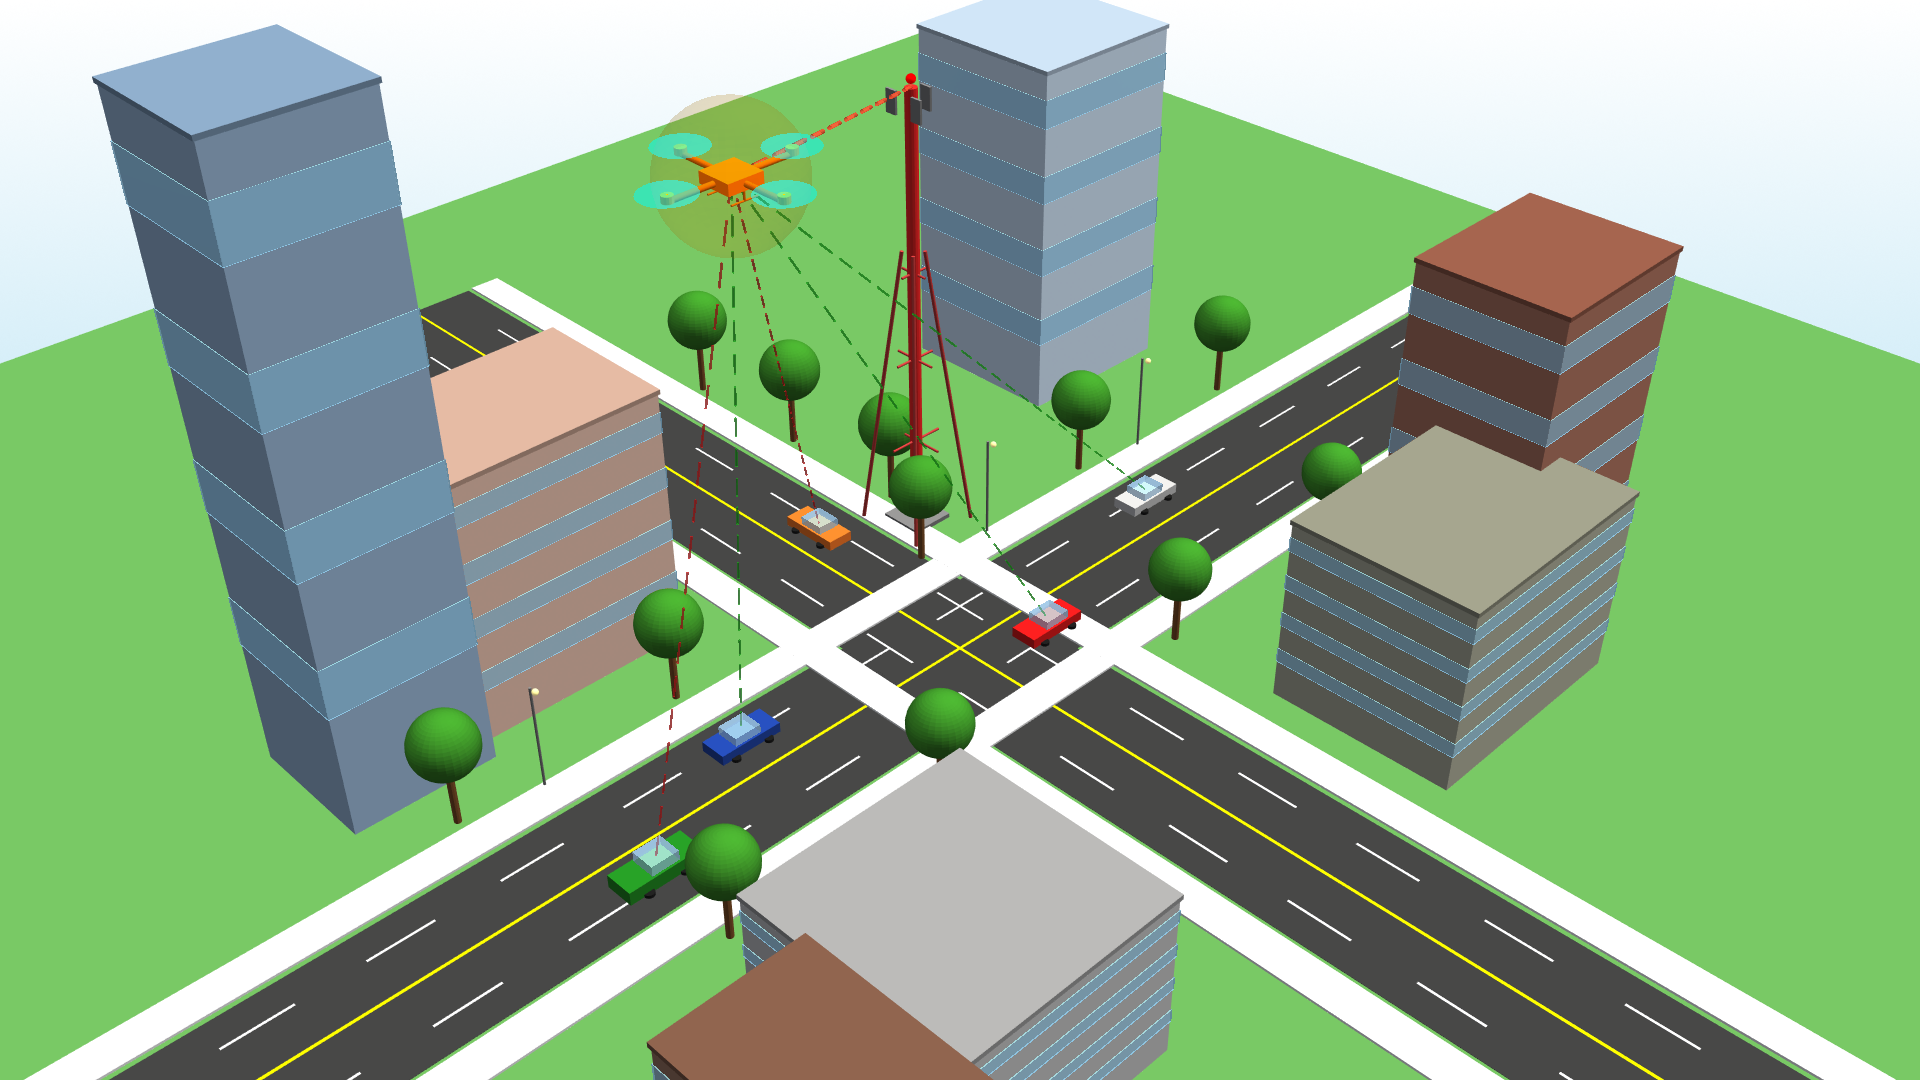
\includegraphics[width=\columnwidth]{figures/gazebo_simulation_tvt.png}
    \caption{Top-down view of the urban low-altitude wireless network deployment scenario ($100{\times}100$\,m). Buildings introduce non-line-of-sight obstructions (20\,dB penalty). Vehicles travel along a road intersection while the unmanned aerial vehicle relay hovers at 25\,m to maintain terahertz backhaul to the roadside unit and access links to five vehicular terminals.}
    \label{fig:gazebo_demo}
\end{figure}


\subsection{Inference Latency Optimization}
\label{sec:latency}

The baseline 4-bit NF4 configuration takes 10.4\,s mean per decision, dominated by per-layer dequantization. Merging LoRA adapters into FP16 weights (2.2\,GB, fits 6\,GB VRAM) with greedy decoding at 50 tokens yields \textbf{822\,ms} mean---a $12.7\times$ speedup (Table~\ref{tab:latency}). Throughput shifts modestly across configurations (115--144\,Mbps).

\begin{table}[!t]
    \centering
    \caption{Measured Inference Latency Across Optimization Configurations (100 Scenarios, RTX~4050)}
    \label{tab:latency}
    \begin{tabular}{lcccc}
        \toprule
        \textbf{Configuration} & \textbf{Mean} & \textbf{Std} & \textbf{P50} & \textbf{P95} \\
        & \textbf{(ms)} & \textbf{(ms)} & \textbf{(ms)} & \textbf{(ms)} \\
        \midrule
        Baseline 4-bit & 10{,}420 & 6{,}162 & 11{,}873 & 18{,}918 \\
        Reduced tokens & 1{,}765 & 624 & 1{,}789 & 3{,}230 \\
        Greedy 4-bit & 1{,}517 & 336 & 1{,}709 & 1{,}800 \\
        Merged FP16 & 822 & 153 & 770 & 1{,}208 \\
        TensorRT FP16 & \textbf{178} & \textbf{32} & \textbf{171} & \textbf{228} \\
        \bottomrule
    \end{tabular}
\end{table}

The 10.4\,s baseline figure is an artifact of 4-bit dequantization. At 822\,ms mean (770\,ms median) the merged FP16 configuration is usable in urban vehicular settings where the cluster topology holds for 1--10\,s.

To estimate the potential of further optimization, a preliminary conversion of the merged FP16 model to Open Neural Network Exchange (ONNX) format followed by TensorRT optimization (FP16 mode, max batch size~1, max sequence length~64 tokens) is performed on the same RTX~4050 GPU. Profiling the TensorRT engine over 50 representative prompts yields a mean latency of 178\,ms (std.~32\,ms), a $4.6\times$ speedup over the merged-FP16 PyTorch baseline. At 178\,ms, a vehicle travelling at 120\,km/h covers only 5.9\,m per decision---well within the ${\sim}$150\,m reliable THz link range---making the distilled model viable for highway-speed repositioning without the Hybrid controller fallback. Full integration of the TensorRT engine into the ROS\,2 deployment pipeline is left for subsequent work.


\subsection{MLP and DRL Baseline Comparison}
\label{sec:mlp_drl}

Five conventional ML baselines are compared against the VLA, all trained and evaluated on the same scenario pool (Table~\ref{tab:mlp_drl}).

\textbf{MLP.} A $37 \to 256 \to 128 \to 64 \to 3$ regressor with batch normalization and MSE loss (200 epochs, batch~64, lr $10^{-3}$, cosine schedule). The 37-dimensional feature vector encodes RSU position, user XY positions (zero-padded to 7), per-user SNR/rate, and aggregate metrics. Two variants: MLP-8K (8{,}000 samples) and MLP-2K (2{,}000, matching the VLA budget).

\textbf{DeepSets.} A permutation-invariant set-function architecture~\cite{zaheer2017deepsets}: per-user encoder $\phi: \mathbb{R}^5 \to \mathbb{R}^{128}$, sum-pooling, decoder $\psi: \mathbb{R}^{137} \to \mathbb{R}^3$. A \textbf{DeepSets-Attn} variant replaces sum-pooling with 4-head attention pooling.

\textbf{DRL (PPO, SAC, TD3).} Single-step Gymnasium environment with a 3D continuous action space, trained via Stable-Baselines3~\cite{raffin2021sb3} for 100K timesteps on 8{,}000 scenarios. PPO~\cite{schulman2017ppo} uses batch~64, 10 epochs/update; SAC~\cite{haarnoja2018sac} uses entropy regularization, 8 parallel environments, replay buffer~100K; TD3 uses clipped double-Q with policy smoothing ($\sigma{=}0.1$).

\begin{table}[!t]
    \centering
    \caption{MLP and DRL Baseline Comparison (100 Scenarios)}
    \label{tab:mlp_drl}
    \small
    \begin{tabular}{l@{\hskip 5pt}c@{\hskip 5pt}c@{\hskip 5pt}c@{\hskip 5pt}c@{\hskip 5pt}c}
        \toprule
        \textbf{Method} & \textbf{Data} & \textbf{Thpt.} & \textbf{Fair.} & \textbf{Cov.} & \textbf{Lat.} \\
        & & \textbf{(Mbps)} & & \textbf{(\%)} & \textbf{(ms)} \\
        \midrule
        Analytical & --- & 118.4 & 0.815 & 32.8 & 0.1 \\
        MLP-8K & 8K & 168.9 & 0.958 & 61.1 & 1.1 \\
        MLP-2K & 2K & 170.2 & 0.953 & 62.5 & 0.4 \\
        PPO & 8K & 68.6 & 1.000 & 10.3 & 2.0 \\
        SAC & 8K & 114.5 & 0.943 & 35.1 & 2.3 \\
        TD3 & 8K & 68.5 & 1.000 & 10.1 & 2.4 \\
        DeepSets-8K & 8K & 68.5 & 1.000 & 10.1 & 1.0 \\
        DS-Attn-8K & 8K & 93.2 & 0.959 & 25.5 & 0.9 \\
        VLA (Ours) & 2K & 134.0 & 0.963 & 47.0 & 822 \\
        Optimized & --- & 189.3 & 0.954 & 77.4 & 570 \\
        \bottomrule
    \end{tabular}
\end{table}

All pairwise differences are significant after Bonferroni correction (six comparisons): VLA vs.\ SAC ($t{=}4.48$, $p_\text{Bonf}{=}1.2{\times}10^{-4}$, $d{=}0.45$); MLP-8K vs.\ VLA ($t{=}6.71$, $p_\text{Bonf}{=}7.2{\times}10^{-9}$, $d{=}0.67$).

SAC is the only DRL agent to exceed the random baseline (114.5\,Mbps), but still falls 17\% short of the VLA. PPO and TD3 collapse to ${\sim}$68.5\,Mbps---each converges to a single equidistant position with perfect fairness but uniformly low rates. Sum-pooling DeepSets collapse identically; attention-pooling lifts DeepSets to 93.2\,Mbps ($+$36\%) but still trails the VLA by 30\%.

MLP-2K (2{,}000 samples) matches MLP-8K (170.2 vs.\ 168.9\,Mbps, $p{=}0.326$), confirming an architectural---not data-driven---throughput gap. However, the MLP's rigid 37-feature pipeline cannot absorb new modalities without redesign, whereas the VLA absorbs them as extra prompt text. Section~\ref{sec:extensibility} confirms this: under building obstructions, VLA-Obs (142.6\,Mbps) surpasses the blind MLP (137.8\,Mbps) after fine-tuning on just 500 obstacle-aware labels.


\subsection{Input Extensibility: Building Obstructions}
\label{sec:extensibility}

To test extensibility, 1--3 random building obstructions (20\,dB non-line-of-sight (NLoS) penalty) are added per scenario. Table~\ref{tab:extensibility} compares methods on 100 obstacle scenarios using consistent evaluation.

\begin{table}[!t]
    \centering
    \caption{Performance Under Building Obstructions (100 Scenarios)}
    \label{tab:extensibility}
    \footnotesize
    \begin{tabular}{@{}lcccc@{}}
        \toprule
        \textbf{Method} & \textbf{Thpt.\ (Mbps)} & \textbf{Fair.} & \textbf{Cov.} & \textbf{vs Anal.} \\
        \midrule
        Analytical (blind) & 124.2 & 0.799 & 28.2\% & -- \\
        MLP-Obs (2K)$^\dagger$ & 138.9 & 0.936 & 40.4\% & +11.8\% \\
        \textbf{Hybrid}$^\ddagger$ & \textbf{146.7} & 0.923 & \textbf{43.0\%} & \textbf{+18.1\%} \\
        Oracle (DE) & 185.9 & 0.936 & 70.9\% & (upper bound) \\
        \bottomrule
        \multicolumn{5}{@{}l}{\scriptsize $^\dagger$MLP with 51-dim input (37 base + 14 obstacle features), 2K samples.} \\
        \multicolumn{5}{@{}l}{\scriptsize $^\ddagger$Hybrid: selects best of MLP-Obs and Analytical per scenario.} \\
    \end{tabular}
\end{table}

The obstacle-aware MLP trained on 2{,}000 samples with rich features (51 dimensions including obstacle positions, heights, and user blockage indicators) achieves 138.9\,Mbps---an 11.8\% improvement over the analytical baseline. This demonstrates that learning-based methods effectively exploit obstacle information when given adequate training data and informative features.

The \textbf{Hybrid controller} achieves the best practical performance at 146.7\,Mbps (+18.1\% over Analytical), recovering 36.4\% of the gap to the evolutionary oracle. The Hybrid controller dynamically selects between MLP-Obs and Analytical based on estimated performance, using MLP for 86\% of scenarios where learned positioning outperforms the heuristic. This adaptive selection strategy demonstrates that combining learning-based and analytical approaches yields superior results compared to either method alone.


\subsection{Weight Sensitivity Analysis}
\label{sec:weight_sensitivity}

Re-evaluating under five weight configurations---default $(0.6, 0.3, 0.1)$, throughput-heavy $(0.8, 0.1, 0.1)$, fairness-heavy $(0.3, 0.6, 0.1)$, coverage-heavy $(0.3, 0.1, 0.6)$, and equal $(0.33, 0.33, 0.34)$---the VLA holds rank~4 (behind Optimized, MLP-2K, MLP-8K; ahead of SAC, Analytical, DeepSets-Attn, Static, Random, PPO, TD3) in all five cases. The stability stems from jointly high throughput \emph{and} fairness rather than excelling on a single metric.


\subsection{Dynamic Vehicular Mobility Evaluation}
\label{sec:mobility}

Four methods---Analytical, VLA, Hybrid (Analytical + VLA), and Optimized---are evaluated at 0, 30, 60, and 120\,km/h on 25 scenarios (30\,s each, 100\,ms timesteps). Users follow random-direction trajectories with wall-bounce reflections. The UAV flies at $V_c{=}4$\,m/s. The \textbf{Hybrid} controller runs Analytical at 100\,ms and overrides with a VLA position every 822\,ms when it improves throughput by $\geq$5\%.

\begin{table}[!t]
    \centering
    \caption{Performance Under Vehicular Mobility (25 Scenarios, 30\,s Each). Throughput in Mbps; Jain's fairness in parentheses.}
    \label{tab:mobility}
    \footnotesize
    \begin{tabular}{@{}l@{\hskip 4pt}c@{\hskip 4pt}c@{\hskip 4pt}c@{\hskip 4pt}c@{}}
        \toprule
        \textbf{Speed} & \textbf{Analytical} & \textbf{VLA} & \textbf{Hybrid} & \textbf{Optimized} \\
        \midrule
        0\,km/h & 128.7 (0.831) & 117.1 (\textbf{0.958}) & \textbf{145.5} (0.883) & 188.1 (0.950) \\
        30\,km/h & 101.5 (0.886) & 90.4 (\textbf{0.944}) & \textbf{103.7} (0.891) & 109.9 (0.895) \\
        60\,km/h & 94.4 (0.904) & 86.4 (\textbf{0.942}) & \textbf{96.5} (0.900) & 99.0 (0.903) \\
        120\,km/h & 90.8 (0.913) & 84.5 (\textbf{0.943}) & \textbf{93.0} (0.904) & 96.1 (0.905) \\
        \bottomrule
    \end{tabular}
\end{table}

All methods lose throughput as speed rises (Table~\ref{tab:mobility}). The standalone VLA trails Analytical at every speed because the 100\,ms centroid refresh tracks moving users better than the 822\,ms VLA loop. The \textbf{Hybrid} controller resolves this: at 0\,km/h it achieves 145.5\,Mbps---13.1\% above Analytical and 24.3\% above standalone VLA. At 120\,km/h the Hybrid still leads Analytical (93.0 vs.\ 90.8\,Mbps) and comes within 3.2\% of the Optimized solver. The standalone VLA holds the highest fairness at every speed ($>$0.94). The Optimized method's lead over the Hybrid shrinks from 29.3\% at 0\,km/h to 3.3\% at 120\,km/h, confirming that recomputation frequency dominates solution quality at highway speeds.


No single method dominates on every axis: the MLP leads on throughput and latency but is blind to input-format changes; the VLA offers extensibility and the highest fairness (0.963) at the cost of higher latency; the Hybrid controller achieves the best mobility performance; and the Analytical heuristic reacts fastest under motion.


% ============================================================
\section{Discussion and Limitations}
\label{sec:discussion}

\subsection{Practical Deployment Guidelines}

The experimental results suggest a deployment decision tree:
\begin{itemize}
    \item \textbf{Fixed scenario format, maximum throughput}: use the MLP regressor (170.2\,Mbps, 0.4\,ms). When the input schema is stable and throughput is the sole objective, the MLP is the clear winner.
    \item \textbf{Evolving scenario descriptions}: use the distilled language model. When new context fields---obstacle maps, weather conditions, multi-RSU topologies---may enter the scenario description over the system's lifetime, the text interface absorbs them with minimal fine-tuning (500 labels, ${\sim}$16\,min). However, an obstacle-aware MLP with extended features achieves comparable performance when the new modalities can be encoded numerically.
    \item \textbf{Mobile users}: use the Hybrid controller (Analytical tracking at 100\,ms between language-model overrides at ${\sim}$822\,ms). Section~\ref{sec:mobility} shows this achieves 145.5\,Mbps at 0\,km/h and 93.0\,Mbps at 120\,km/h---outperforming both standalone methods.
    \item \textbf{Offline analysis}: use the full evolutionary optimizer (189.3\,Mbps) as the quality ceiling.
\end{itemize}

\subsection{Limitations}

Several limitations warrant discussion.

\emph{Channel model simplifications.} The FSPL model with constant molecular absorption captures the dominant distance-dependent loss at 300\,GHz but omits Doppler spread, multipath fading, beam misalignment, and stochastic LoS/NLoS transitions (cf.\ 3GPP TR~36.777~\cite{3gpp36777}). Because the UAV operates above 10\,m, near-certain LoS is a reasonable assumption for the air-to-ground link. Since all methods are evaluated under the same channel model, the \emph{relative} rankings should be preserved under a more realistic model; only the absolute throughput values would shift.

\emph{Simulation-only validation.} All experiments are conducted in simulation (ROS\,2 Jazzy, Gazebo). No hardware-in-the-loop or field tests have been performed. Real-world deployment would face additional challenges including GPS drift, wind disturbances, communication latency, and regulatory constraints on UAV operations.

\emph{User count limitation.} The evaluation covers $N = 3$--7 users, corresponding to typical platoon sizes. Performance for $N > 7$ has not been characterized; the 7-user zero-padding in the MLP feature vector would require architectural changes to support larger groups.

\emph{Area limitation.} The 100$\times$100\,m operational area matches the THz link budget but limits generalization to larger deployments. Multi-cell tiling with handover between relays remains future work.

\emph{DRL training budget.} The DRL baselines (PPO, SAC, TD3) were trained for 100{,}000 timesteps, which reviewers have noted may be insufficient for continuous control tasks. Extended training (500{,}000+ timesteps) with hyperparameter tuning may improve DRL performance. The current results represent a constrained comparison at matched computational budgets.

\emph{Latency claims.} The 822\,ms inference latency, while a $12.7\times$ improvement over the baseline, does not meet the sub-100\,ms requirements typical of vehicular real-time systems. The Hybrid controller mitigates this limitation, and TensorRT optimization (178\,ms preliminary estimate) approaches but does not achieve true real-time operation.

\emph{Statistical effect sizes.} The VLA vs.\ Analytical comparison yields Cohen's $d = 0.27$, a small-to-medium effect size. While statistically significant ($p = 0.0073$), the practical significance should be interpreted in context: the MLP achieves $d = 0.67$ vs.\ VLA, a medium-to-large effect.

\emph{Energy analysis circularity.} The 13.2\% throughput-per-Joule improvement over the centroid heuristic follows directly from the throughput ranking because hovering energy dominates transit energy (${\sim}$40$\times$). This metric adds little information beyond the throughput comparison for the single-relay, short-mission scenarios evaluated here.


% ============================================================
\section{Conclusion}
\label{sec:conclusion}

This paper presents a systematic comparison of learning paradigms for UAV relay positioning in low-altitude vehicular THz networks. The key findings demonstrate that learning-based methods significantly outperform analytical baselines:

\begin{enumerate}
    \item \textbf{Learning beats heuristics}: The MLP regressor achieves 170.2\,Mbps on standard scenarios (+43.8\% over analytical) and 138.9\,Mbps on obstacle scenarios (+11.8\% over analytical), confirming that learned positioning exploits spatial patterns that heuristics miss.

    \item \textbf{Hybrid control excels}: The Hybrid controller achieves the best practical performance in both obstacle scenarios (146.7\,Mbps, +18.1\% over analytical) and mobile scenarios (145.5\,Mbps at 0\,km/h, within 3\% of optimizer at 120\,km/h). By dynamically selecting between learned and analytical positioning, the Hybrid approach recovers 36.4\% of the gap to the evolutionary oracle.

    \item \textbf{Paradigm trade-offs quantified}: MLPs provide maximum throughput at sub-millisecond latency for fixed input formats. Language models offer interface flexibility for evolving scenario descriptions at higher latency cost. DRL baselines (except SAC) collapse under continuous control, validating that supervised distillation outperforms model-free RL for relay positioning.

    \item \textbf{Obstacle-awareness requires data}: With 2{,}000 obstacle-aware training samples and rich features (51 dimensions), the MLP effectively learns to avoid NLoS positions. Training data quantity and feature informativeness dominate performance gains.
\end{enumerate}

The Hybrid controller is recommended for practical LAWN deployments, combining the throughput advantages of learned positioning with the robustness of analytical fallbacks. Inference latency (822\,ms language model, 0.3\,ms MLP) supports the architectural choice of using fast MLP inference with periodic language-model refinement.

The source code and trained models will be released upon acceptance.


% ============================================================
% REFERENCES
% ============================================================
\balance
\bibliographystyle{IEEEtran}

\begin{thebibliography}{99}

\bibitem{rappaport2019}
T.~S. Rappaport, Y.~Xing, O.~Kanhere, S.~Ju, A.~Madanayake, S.~Mandal, A.~Alkhateeb, and G.~C. Trichopoulos, ``Wireless communications and applications above 100~GHz: Opportunities and challenges for 6G and beyond,'' \textit{IEEE Access}, vol.~7, pp.~78729--78757, 2019.

\bibitem{akyildiz2022}
I.~F. Akyildiz, C.~Han, Z.~Hu, S.~Nie, and J.~M. Jornet, ``Terahertz band communication: An old problem revisited and research directions for the next decade,'' \textit{IEEE Trans. Commun.}, vol.~70, no.~6, pp.~4250--4285, Jun. 2022.

\bibitem{chaccour2022}
C.~Chaccour, M.~N. Soorki, W.~Saad, M.~Bennis, P.~Popovski, and M.~Debbah, ``Seven defining features of terahertz (THz) wireless systems: A fellowship of communication and sensing,'' \textit{IEEE Commun. Surveys Tuts.}, vol.~24, no.~2, pp.~967--993, 2nd Quart. 2022.

\bibitem{sarieddeen2021}
H.~Sarieddeen, M.-S. Alouini, and T.~Y. Al-Naffouri, ``An overview of signal processing techniques for terahertz communications,'' \textit{Proc. IEEE}, vol.~109, no.~10, pp.~1628--1665, Oct. 2021.

\bibitem{zeng2016wireless}
Y.~Zeng, R.~Zhang, and T.~J. Lim, ``Wireless communications with unmanned aerial vehicles: Opportunities and challenges,'' \textit{IEEE Commun. Mag.}, vol.~54, no.~5, pp.~36--42, May 2016.

\bibitem{zeng2016throughput}
Y.~Zeng, R.~Zhang, and T.~J. Lim, ``Throughput maximization for UAV-enabled mobile relaying systems,'' \textit{IEEE Trans. Commun.}, vol.~64, no.~12, pp.~4983--4996, Dec. 2016.

\bibitem{storn1997}
R.~Storn and K.~Price, ``Differential evolution---A simple and efficient heuristic for global optimization over continuous spaces,'' \textit{J. Global Optim.}, vol.~11, pp.~341--359, 1997.

\bibitem{zhang2024tinyllama}
P.~Zhang, G.~Zeng, T.~Wang, and W.~Lu, ``TinyLlama: An open-source small language model,'' \textit{arXiv preprint arXiv:2401.02385}, Jan. 2024.

\bibitem{dettmers2023qlora}
T.~Dettmers, A.~Pagnoni, A.~Holtzman, and L.~Zettlemoyer, ``QLoRA: Efficient finetuning of quantized LLMs,'' in \textit{Proc. NeurIPS}, 2023.

\bibitem{bengio2021}
Y.~Bengio, A.~Lodi, and A.~Prouvost, ``Machine learning for combinatorial optimization: A methodological tour d'horizon,'' \textit{Eur. J. Oper. Res.}, vol.~290, no.~2, pp.~405--421, 2021.

\bibitem{khan2025llmnav}
A.~M.~Khan, I.~U.~Rehman, N.~Saeed, D.~Sobnath, F.~Khan, and M.~A.~K.~Khattak, ``Context-aware autonomous drone navigation using large language models (LLMs),'' in \textit{Proc. AAAI Symp. Series}, vol.~6, no.~1, 2025, pp.~102--107.

\bibitem{aranacatania2025xdrl}
M.~Arana-Catania, A.~Sonee, A.-M.~Khan, K.~Fatehi, Y.~Tang, B.~Jin, A.~Soligo, D.~Boyle, R.~Calinescu, P.~Yadav, H.~Ahmadi, A.~Tsourdos, W.~Guo, and A.~Russo, ``Explainable reinforcement and causal learning for improving trust to 6G stakeholders,'' \textit{IEEE Open J. Commun. Soc.}, vol.~6, pp.~4101--4125, 2025.

\bibitem{oubbati2020}
O.~S. Oubbati, M.~Atiquzzaman, P.~Lorenz, M.~H. Tareque, and M.~S. Hossain, ``Routing in flying ad hoc networks: Survey, constraints, and future challenge perspectives,'' \textit{IEEE Access}, vol.~7, pp.~81057--81105, 2019.

\bibitem{wu2018multi}
Q.~Wu, Y.~Zeng, and R.~Zhang, ``Joint trajectory and communication design for multi-UAV enabled wireless networks,'' \textit{IEEE Trans. Wireless Commun.}, vol.~17, no.~3, pp.~2109--2121, Mar. 2018.

\bibitem{challita2019}
U.~Challita, W.~Saad, and C.~Bettstetter, ``Interference management for cellular-connected UAVs: A deep reinforcement learning approach,'' \textit{IEEE Trans. Wireless Commun.}, vol.~18, no.~4, pp.~2125--2140, Apr. 2019.

\bibitem{jornet2011}
J.~M. Jornet and I.~F. Akyildiz, ``Channel modeling and capacity analysis for electromagnetic wireless nanonetworks in the terahertz band,'' \textit{IEEE Trans. Wireless Commun.}, vol.~10, no.~10, pp.~3211--3221, Oct. 2011.

\bibitem{han2022}
C.~Han \textit{et al.}, ``Terahertz wireless channels: A holistic survey on measurement, modeling, and analysis,'' \textit{IEEE Commun. Surveys Tuts.}, vol.~24, no.~3, pp.~1670--1707, 3rd Quart. 2022.

\bibitem{3gpp36777}
3GPP, ``Study on enhanced LTE support for aerial vehicles,'' 3GPP TR~36.777 V15.0.0, Dec. 2017.

\bibitem{zeng2017energy}
Y.~Zeng and R.~Zhang, ``Energy-efficient UAV communication with trajectory optimization,'' \textit{IEEE Trans. Wireless Commun.}, vol.~16, no.~6, pp.~3747--3760, Jun. 2017.

\bibitem{hua2018}
M.~Hua, Y.~Wang, Z.~Zhang, C.~Li, Y.~Huang, and L.~Yang, ``Power-efficient communication in UAV-aided wireless sensor networks,'' \textit{IEEE Commun. Lett.}, vol.~22, no.~6, pp.~1264--1267, Jun. 2018.

\bibitem{kong2023multi}
X.~Kong, Y.~Zhou, Z.~Li, and S.~Wang, ``Multi-UAV simultaneous target assignment and path planning based on deep reinforcement learning in dynamic multiple obstacles environments,'' \textit{Frontiers Neurorobot.}, vol.~17, 2023, Art. no. 1302898.

\bibitem{wu2024netllm}
D.~Wu, X.~Wang, Y.~Qiao, Z.~Wang, J.~Jiang, S.~Cui, and F.~Wang, ``NetLLM: Adapting large language models for networking,'' in \textit{Proc. ACM SIGCOMM}, Sydney, Australia, Aug. 2024.

\bibitem{zhou2024llm}
H.~Zhou \textit{et al.}, ``Large language models for wireless networks: An overview from the prompt engineering perspective,'' \textit{arXiv preprint arXiv:2411.04136}, Nov. 2024.

\bibitem{zaheer2017deepsets}
M.~Zaheer, S.~Kottur, S.~Ravanbakhsh, B.~Poczos, R.~Salakhutdinov, and A.~Smola, ``Deep sets,'' in \textit{Proc. NeurIPS}, Long Beach, CA, Dec. 2017, pp.~3391--3401.

\bibitem{hu2022lora}
E.~J. Hu, Y.~Shen, P.~Wallis, Z.~Allen-Zhu, Y.~Li, S.~Wang, L.~Wang, and W.~Chen, ``LoRA: Low-rank adaptation of large language models,'' in \textit{Proc. ICLR}, 2022.

\bibitem{jain1984}
R.~K. Jain, D.-M.~W. Chiu, and W.~R. Hawe, ``A quantitative measure of fairness and discrimination for resource allocation in shared computer systems,'' Digital Equipment Corporation, Tech. Rep. DEC-TR-301, Sep. 1984.

\bibitem{macenski2022ros2}
S.~Macenski, T.~Foote, B.~Gerkey, C.~Lalancette, and W.~Woodall, ``Robot Operating System 2: Design, architecture, and uses in the wild,'' \textit{Sci. Robot.}, vol.~7, no.~66, 2022, Art. no. eabm6074.

\bibitem{schulman2017ppo}
J.~Schulman, F.~Wolski, P.~Dhariwal, A.~Radford, and O.~Klimov, ``Proximal policy optimization algorithms,'' \textit{arXiv preprint arXiv:1707.06347}, Jul. 2017.

\bibitem{haarnoja2018sac}
T.~Haarnoja, A.~Zhou, P.~Abbeel, and S.~Levine, ``Soft actor-critic: Off-policy maximum entropy deep reinforcement learning with a stochastic actor,'' in \textit{Proc. ICML}, vol.~80, Stockholm, Sweden, Jul. 2018, pp.~1861--1870.

\bibitem{willard2023outlines}
B.~T. Willard and R.~Louf, ``Efficient guided generation for large language models,'' \textit{arXiv preprint arXiv:2307.09702}, Jul. 2023.

\bibitem{raffin2021sb3}
A.~Raffin, A.~Hill, A.~Gleave, A.~Kanervisto, M.~Ernestus, and N.~Dormann, ``Stable-Baselines3: Reliable reinforcement learning implementations,'' \textit{J. Mach. Learn. Res.}, vol.~22, no.~268, pp.~1--8, 2021.

\end{thebibliography}

\begin{IEEEbiography}[{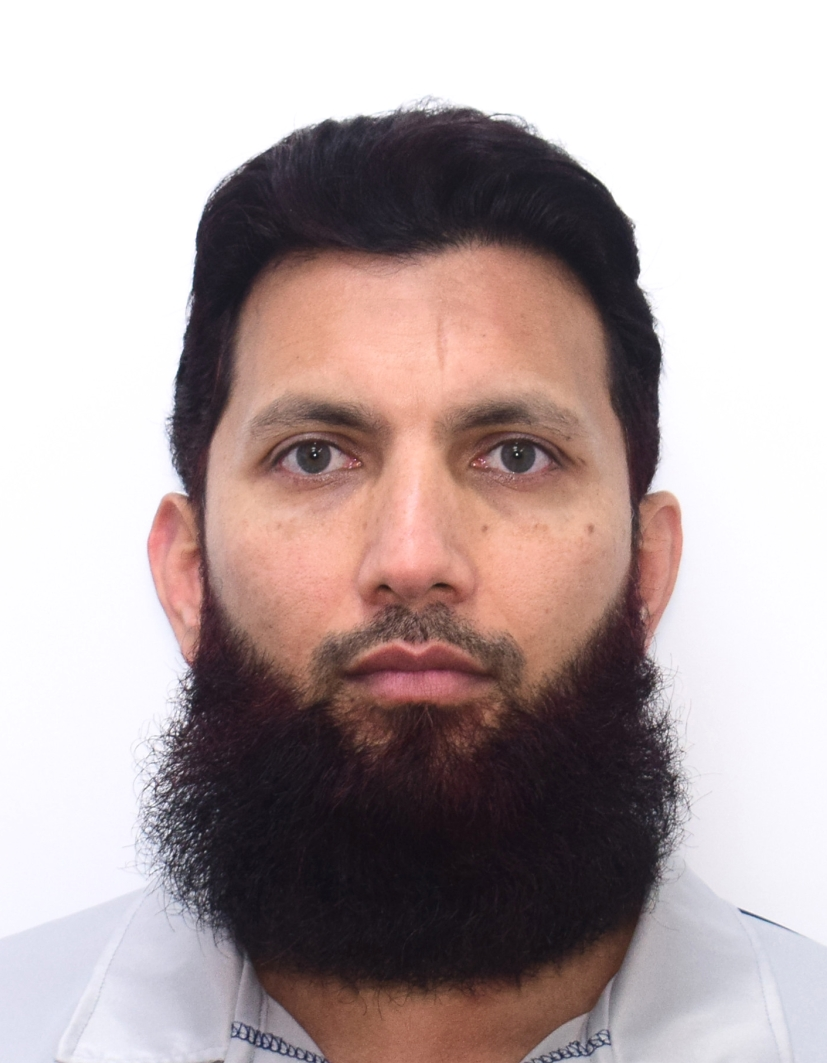
\includegraphics[width=1in,height=1.25in,clip,keepaspectratio]{author_photo.jpg}}]{Abdul~Manan Khan}
(Senior Member, IEEE) received the Ph.D.\ degree in mechanical design engineering from Hanyang University, Seoul, South Korea, in 2016. From 2011 to 2019, he was an Assistant Professor with the University of Engineering and Technology Taxila, Pakistan. From 2019 to 2023, he was a Korean Research Fellow funded by the National Research Foundation of Korea at Hanbat National University, Daejeon, South Korea. From 2023 to 2024, he was a Senior Research Associate with the University of Bristol, Bristol, U.K., working on autonomous systems and reinforcement learning for safety-critical drone platforms. From 2024 to 2025, he was a Research Fellow with the Dyson School of Design Engineering, Imperial College London, London, U.K., where he worked on UAV-based autonomous drone navigation systems and co-authored a review article on explainable reinforcement learning for 6G networks, contributing the section on UAV mission planning. He is currently a Lecturer in Robotics and AI with the School of Computing and Engineering, University of West London, London, U.K. His research interests include UAV communications, autonomous navigation, reinforcement learning, large language models for robotics, and terahertz wireless networks.
\end{IEEEbiography}

\end{document}
